\documentclass{article}
\usepackage[utf8]{inputenc}

\usepackage{amsmath}
\usepackage{amsfonts}

\usepackage{hyperref}
\hypersetup{
    colorlinks=true,
    linkcolor=blue,
    filecolor=magenta,      
    urlcolor=cyan,
}

\usepackage{graphicx}

\setlength{\parindent}{0pt}

\title{Assignment-1 : LARP}
\author{Sankaran Vaidyanathan and Karthik Thiagarajan (CS16S027)}

\begin{document}

\maketitle

\tableofcontents

\newpage
\section{Question-2}

\subsection{Part-a}

\textbf{Observations}
\begin{figure}[h!]
	\centering
	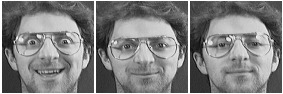
\includegraphics[width=0.6\textwidth]{images/faces/face256}
	\caption{Faces 2, 5 and 6}
\end{figure}

\begin{figure}[h!]
	\centering
	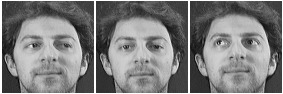
\includegraphics[width=0.6\textwidth]{images/faces/face8910}
	\caption{Faces 8, 9 and 10}
\end{figure}

\begin{figure}[h!]
	\centering
	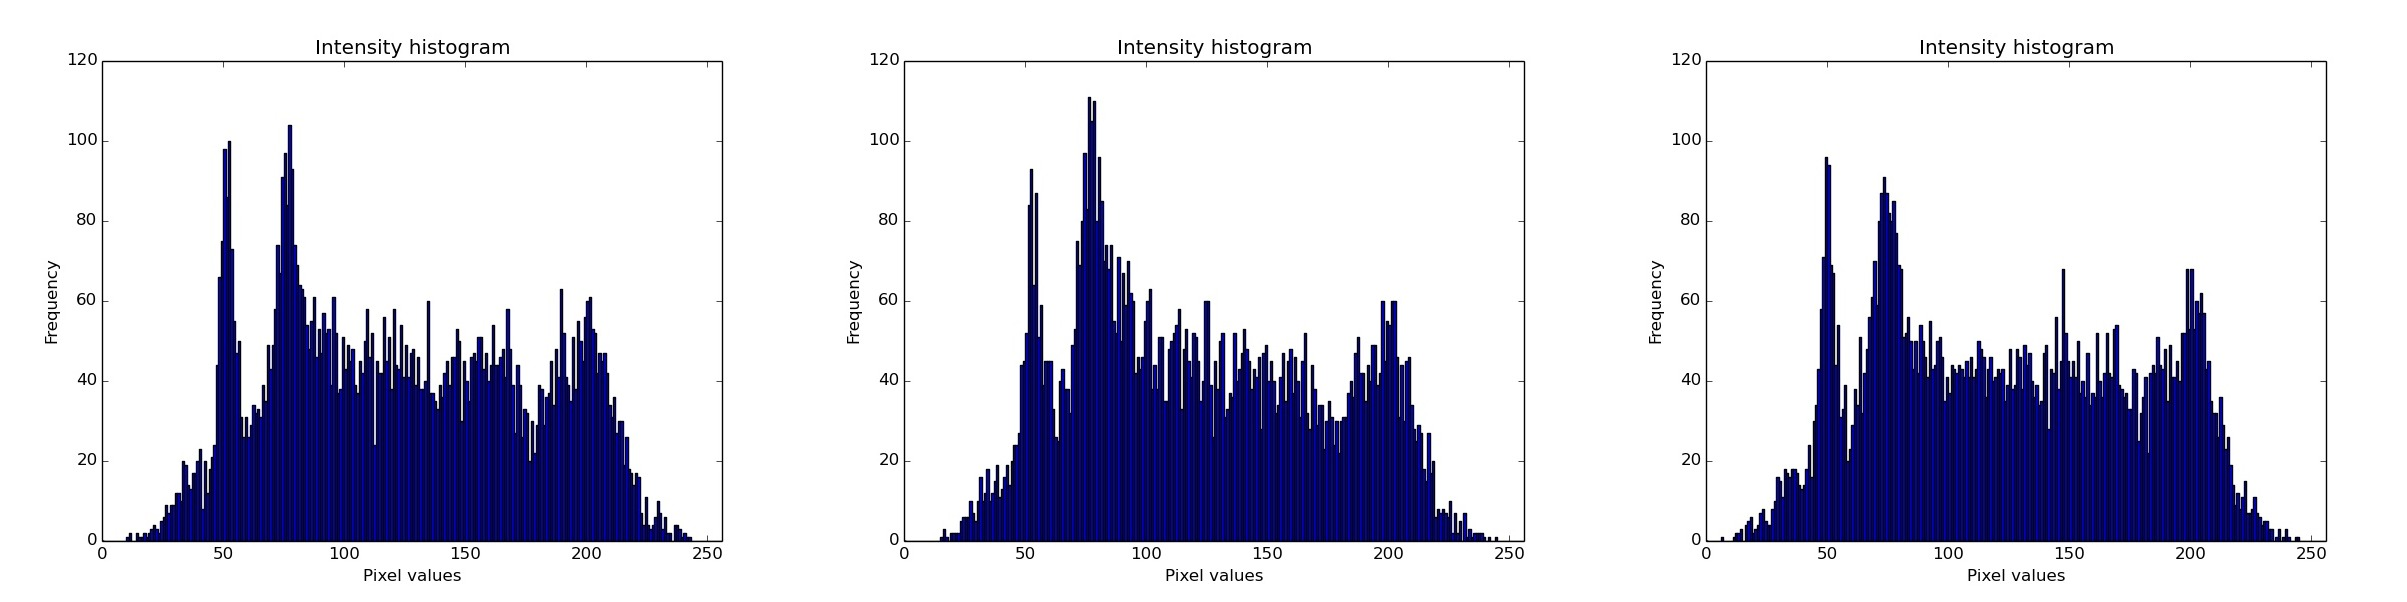
\includegraphics[width=\textwidth]{images/hists/face256}
	\caption{Faces 2, 5 and 6}
\end{figure}

\begin{figure}[h!]
	\centering
	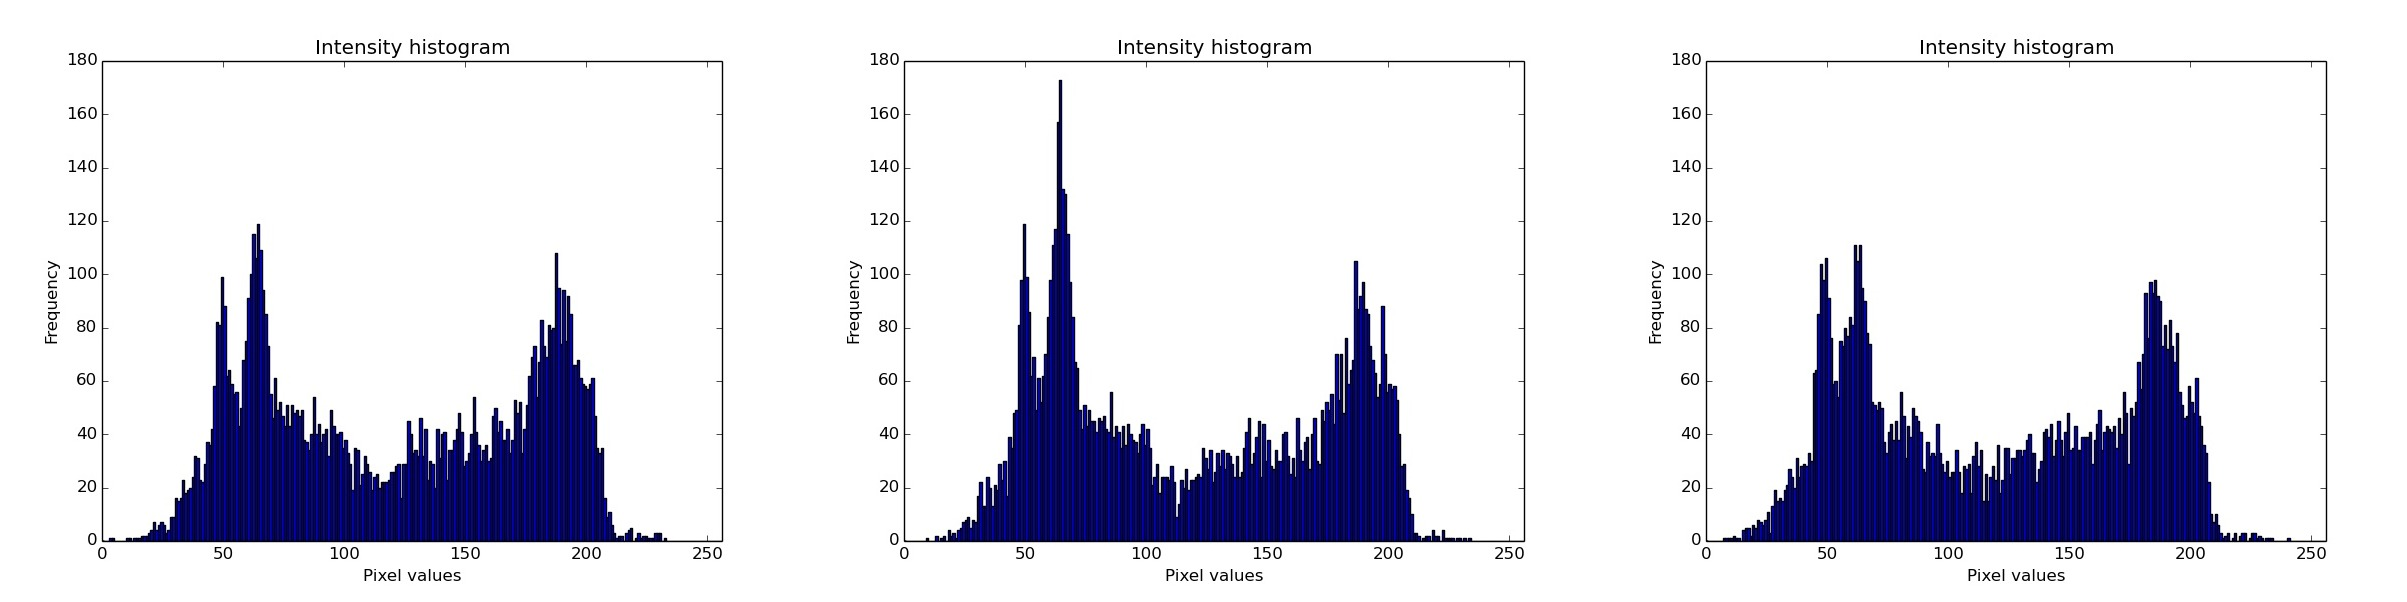
\includegraphics[width=\textwidth]{images/hists/face8910}
	\caption{Faces 8, 9 and 10}
\end{figure}

\newpage


\textbf{Inference}\\
All ten images look very similar and the intensity histograms reflect this similarity. In general, the intensity distribution has three peaks, one centred at 200, the other two occurring near the intensity value of 50.
There is an interesting observation concerning faces with glasses. The distribution is quite uniform between the left and right peaks. Contrast this with the distribution of the faces without glasses - there is a clear valley between the peaks. Though the global shape of the intensity distribution is the same across all ten images, there are subtle local variations. These variations are identical for images that are similar to each other. ``Wearing glasses" is one notion of similarity.

\newpage
\subsection{Part-b}

\textbf{Flesh, Blood and Bone}\\

Before looking at the basis vectors, it is essential to understand the process used to generate them. The reason will become clear as we go along. Let us assume that we are working with a collection of $N$ face images. Each image is a $92 \times 92$ matrix, and can be converted to an $8464$ dimensional vector. To begin with, we assume that the  vectorization proceeds row-wise. 
\begin{align*}
\mu &= \frac{1}{N} \sum \limits_{i = 1}^{N} f_{i}\\
\Sigma &= \frac{1}{N} \sum \limits_{i = 1}^{N} (f_{i} - \mu)(f_{i} - \mu)^{T}\\
\Sigma &= Q \Lambda Q^{T}
\end{align*}

, where $f_i$ is the $i^{th}$ face-vector, $\mu$ is the estimated mean and $\Sigma$ is the estimated covariance matrix. $\Sigma$ is an $8464 \times 8464$ symmetric matrix. By the spectral theorem, we can find a basis for $\mathbb{R}^{8464}$ consisting of orthonormal eigenvectors of $\Sigma$. $Q$ is the matrix whose columns are these eigenvectors. We have been given this matrix to work with.

When an eigenvector is extracted from $Q$ and reshaped to $92 \times 92$, we observe that the resulting image - called an eigenface in computer vision literature - is rotated 90 degrees anti-clockwise. Clearly, the order of reshaping is different. MATLAB uses the Fortran ordering to reshape matrices. NumPy uses the C ordering. By explicitly specifying the Fortran ordering, we get the correct eigenfaces.

\begin{figure}[h!]
	\centering
	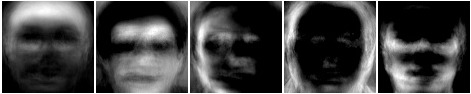
\includegraphics[width=\textwidth]{images/eigfaces/face0-4}
	\caption{Flesh : Eigenfaces 1 to 5}
\end{figure}

\begin{figure}[h!]
	\centering
	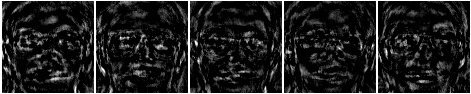
\includegraphics[width=\textwidth]{images/eigfaces/face100-104}
	\caption{Bone : Eigenfaces 101 to 105}
\end{figure}

\begin{figure}[h!]
	\centering
	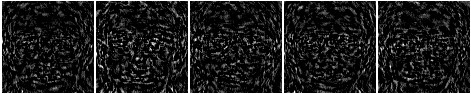
\includegraphics[width=\textwidth]{images/eigfaces/face300-304}
	\caption{Blood : Eigenfaces 301 to 305}
\end{figure}

\begin{figure}[h!]
	\centering
	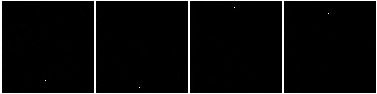
\includegraphics[width=\textwidth]{images/eigfaces/facenoise}
	\caption{Pixel-faces : Eigenfaces beyond 400}
\end{figure}

\end{document}